%%%%%%%%%%%%%%%%%%%%%%%%%%%%%%%%%%%%%%%%%%%%%%%%%%%%%%%%%%%%%%%%%%%%%%%%%%%%%
%% MS Draft Journal of Ecology Special Issue, Dispersal - SUPPL MATERIAL
%% Pedro - 07 June 2016
%----------------------------------------------------------------------------
%%%%%%%%%%%%%%%%%%%%%%%%%%%%%%%%%%%%%%%%%%%%%%%%%%%%%%%%%%%%%%%%%%%%% Headers
\documentclass[a4paper, 12pt]{article}
\usepackage{graphicx}
\usepackage[utf8]{inputenc}
\usepackage[a4paper]{geometry}
\usepackage{hyperref}
\pagestyle{plain}
\usepackage{amsmath,amssymb}
\usepackage{geometry}
\usepackage{lscape}
\usepackage{setspace}
\usepackage{verbatim}
\usepackage{graphicx}
\usepackage{epstopdf}
\usepackage{booktabs}
\usepackage{natbib}
\usepackage{longtable}
\usepackage{rotating}                                                                                     
\newcommand{\tab}{\hspace{5mm}}
\usepackage{tabularx} 
\usepackage[margin=10pt,font=small,labelfont=bf]{caption}
\usepackage[left]{lineno}
\usepackage{caption}
\DeclareGraphicsRule{.tif}{png}{.png}{`convert #1 `basename #1 .tif`.png}
\usepackage{fancyhdr} % This should be set AFTER setting up the page geometry
\pagestyle{empty}     % options: empty , plain , fancy
\renewcommand{\headrulewidth}{0pt} % customise the layout...
\lhead{{\tiny Jordano - What is long-distance dispersal?}}\chead{}\rhead{}
\lfoot{}\cfoot{\thepage}\rfoot{}
\usepackage{parskip}
\linespread{1.25}
%%%%%%%%%%%%%%%%%%%%%%%%%%%%%%%%%%%%%%%%%%%%%%%%%%%%%%%%%%%%%%%%%% Title page
\begin{document}


\title{Manuscript Draft\\
\vspace{2cm}
What is long-distance dispersal? And a taxonomy of dispersal events \\
\textbf{Supplementary Material}}

\author{Pedro Jordano$^{\dag}$}

\date{Sevilla, \today}
\maketitle


\begin{spacing}{1.0}
$^{\dag}$ {\small Integrative Ecology Group, Estaci\'on Biol\'ogica de 
Do\~nana, CSIC, Avda. Americo Vespucio, s/n, Isla de La Cartuja
E-41092 Sevilla, Spain.}\\


{\small \textit{Corresponding author:} Pedro Jordano. Integrative Ecology Group, Estaci\'on Biol\'ogica de Do\~nana, CSIC, Avda. americo Vespucio, s/n, E-41092 Sevilla, Spain. Email address: jordano@ebd.csic.es}\\

\textbf{Key words}: ***\\

{\small \textbf{Manuscript information: }** Words; ** Chars; ** Pages, * Figures; * Tables.}
\end{spacing}

\maketitle
\newpage

%-------------------------------------------------------------------- METHODS
\begin{linenumbers}

\section*{Methods}

\paragraph*{Species and Study Site.} The tree species we use as a case study to illustrate different types of dispersal events, \textit{Prunus mahaleb} (L.) (Rosaceae), is a shrub or small tree that produces fleshy fruits that are consumed by frugivores, who disperse seeds after regurgitating or defecating them. This species is frequently visited during July to mid-August by small- and medium-sized birds and carnivorous mammals that include fruits in their diets during late summer to winter \citep{Jordano:2000ft}. \textit{P. mahaleb} occurs in a patchy distribution at the regional scale, with relatively isolated populations consisting of dozens to hundreds of trees. Our study population included a total of 196 adult reproductive trees distributed over an area of 26 ha in patches of variable density. Other populations within 20 km exist as scattered patches of 10–150 trees, with some containing $\geqq$ 1,000 trees. The nearest population is 1.5 km away. Additional information on the study population and description of methodological apporaches is reported by \citet{Jordano:2007} and \citet{Garcia:2009do} and references therein.

\paragraph*{Sampling dispersed seeds.} 
To estimate the relative contribution of each dispersal vector to the different categories of dispersal events defined in Table 1, we first collected dispersed seeds, following different sampling schemes according to the functional group of dispersal vector. We used this grouping of frugivores giving the difficulties of resolving the identification of scats, pellets and regurgitated seeds down to species level just based on visual cues. We differentiated four major frugivore types: large carnivorous mammals (such as foxes, badgers, and stone martens); two species of medium- and large-sized frugivorous birds, mistle thrushes (\textit{T. viscivorus}), and carrion crows (\textit{C. corone}); and a pool of small-sized frugivorous birds, including warblers, redstarts, and robins \citep{Jordano:2007}. 

Seeds were collected in 1997–1999 and 2003–2005. The sampling schemes are described in detail elsewhere \citep{Jordano:2007,Garcia:2009do} and include a combination of seed traps and direct sampling of mammal feces along fixed transects. We haphazardly collected 130 samples of mammal feces during the \textit{P. mahaleb} fruit ripening period and recorded their location relative to potential source trees. Overall, we genotyped 167 seeds from 20 fecal samples. Most samples were from red fox (\textit{Vulpes vulpes}) and stone marten (\textit{Martes foina}); some ( 10 samples) were from badger (\textit{Meles meles}) \citep{Jordano:2007}.

In addition we sampled directly the pellets of large corvids (\textit{Corvus corone}) and from \textit{Turdus viscivorus}, the latter by direct sampling beneath pine trees and scats from seed traps \citep[see ][ for details]{Jordano:2007}. Finally, a seed sample directly from seed traps included seeds dispersed by small- and medium-sized passerines, such as \textit{Phoenicurus ochruros}, \textit{Turdus merula}, \textit{Erithacus rubecula}, \textit{Sylvia communis}, \textit{Sylvia atricapilla}, etc. \citep{Jordano:2007}. The total seed sample thus consisted of seed endocarps collected from the seed traps (mostly small passerines) ($n= $465), mammal scats ($n= $167), and \textit{C. corone} pellets ($n= $23) \citep[see Table 1 in ][]{Jordano:2007}. 

\paragraph*{Seed genotyping.} 
We used material described in \citet{Jordano:2007}, and genotyping methods described in detail in previous work \citep{Godoy:2001,Garcia:2007he,Garcia:2009do}. Briefly, we used a set of 10 polymorphic microsatellite markers (simple DNA sequence repeats) \citep{Godoy:2001} to obtain the multilocus genotypes of both of the adult trees (candidate source trees from the study population) and the sample of seed endocarps. Given that all adult trees in the population had a distinct multilocus genotype, an unambiguous assignment of each seed to its source tree could be made. When a full match between the endocarp genotype and any of the adult-tree genotypes in the population was not possible, we assumed that the seed came from another population. To assess the effect of genotyping errors, we reexamined the exclusion of genotypes due to a single locus mismatch, two loci mismatches, etc. At the analysis level, any exclusion of identity between a seed and a potential mother tree based on mismatches of only one or two loci was rechecked. We used GIMLET software \citep{Valiere:2002fo} to find the matching adult multilocus genotype for each endocarp with eight or more loci successfully typed. Because each seed belonged to one of the four groups of dispersers, we could thus derive the relative contribution of each frugivore group to different classes of seed dispersal events and to seed immigration.

\paragraph*{Contribution of dispersal vectors to types of dispersal events.} 
We considered each dispersed seed as an independent replicate, because each represented a dispersal event from the perspective of plant population genetics, i.e., an independent "arrival" event resulting from the dispersal process mediated by the frugivore. 

Once the maternal source tree of each individual seed was identified (or its provenance from outside the study population determined) we assessed the dispersal distance and grouped the seeds separately as coming from trees located within or outside the population. In addition, for seeds originating from local trees we determined whether dispersal distances were $\geqq$ 45 m to sort out $LDD_{loc}$ dispersal events from $SDD_{loc}$ events. All the events involving immigrant seeds were considered $LDD_{ss}$ by definition, given that the neighborhood size was very reduced (radius= 0.045 km) relative to the geographic limits of the study population (maximum length for a within-population dispersal event: 1220 m)\citep{Garcia:2009do}. Along this reasoning, $LDD_{neigh}$ events were considered non-existent in this particular case study given that neighborhood size area was smaller than the population area.

\end{linenumbers}
\newpage

%%%%%%%%%%%%%%%%%%%%%%%%%%%%%%%%%%%%%%%%%%%%%%%%%%%%%% Supplementary Material
%------------------------------------------------------------------- Table S1
\begin{landscape}
\begin{table}
  \caption*{Table S1. Summary of neighborhood area sizes and estimated neighborhood radius for tree species with different combinations of dispersal modes. Data from \citet{Nason:1998aa,Garcia:2005fu,Garcia:2007he} and present study.}
  \vspace{0.5cm}
    \begin{tabular}{lllccc}
        \hline \\
     Species                & Pollinator  & Seed disperser & Density ($ha^{-1}$) & Breeding unit ($km^2$) & Radius (km) \\\\ \hline \\
    \textit{Ficus dugandii}          & Fig wasp    & Vertebrates    & 0.004          & 631.7               & 14.2        \\
    \textit{Ficus obtusifolia}       & Fig wasp    & Vertebrates    & 0.072          & 105.9               & 5.8         \\
    \textit{Prunus mahaleb}          & Bees, flies & Vertebrates    & 0.003          & 0.87                & 0.042       \\
    \textit{Frangula alnus}          & Bees, flies & Vertebrates    & 0.0004         & 0.45                & 0.013       \\
    \textit{Astrocaryum mexicanum}   & Beetle      & Vertebrates    & 1364.0         & 0.011               & 0.06        \\
    \textit{Calophyllum longifolium} & Bees        & Vertebrates    & 0.28           & 1.241               & 0.629       \\
    \textit{Platypodium elegans}     & Bees        & Wind           & 0.78           & 0.866               & 0.525       \\
    \textit{Cedrus atlantica}        & Wind        & Wind           & 61.7           & 0.151               & 0.22        \\
   \textit{Fraxinus americana}      & Wind        & Wind           & 24.7           & 0.008               & 0.05        \\
    \textit{Pseudotsuga menziesii}   & Wind        & Wind           & 25.0           & 0.078               & 0.158       \\\\
\hline
    \end{tabular}
\end{table}
\end{landscape}
\newpage 

%------------------------------------------------------------------ Figure S1
\begin{figure}[htbp]
\centerline{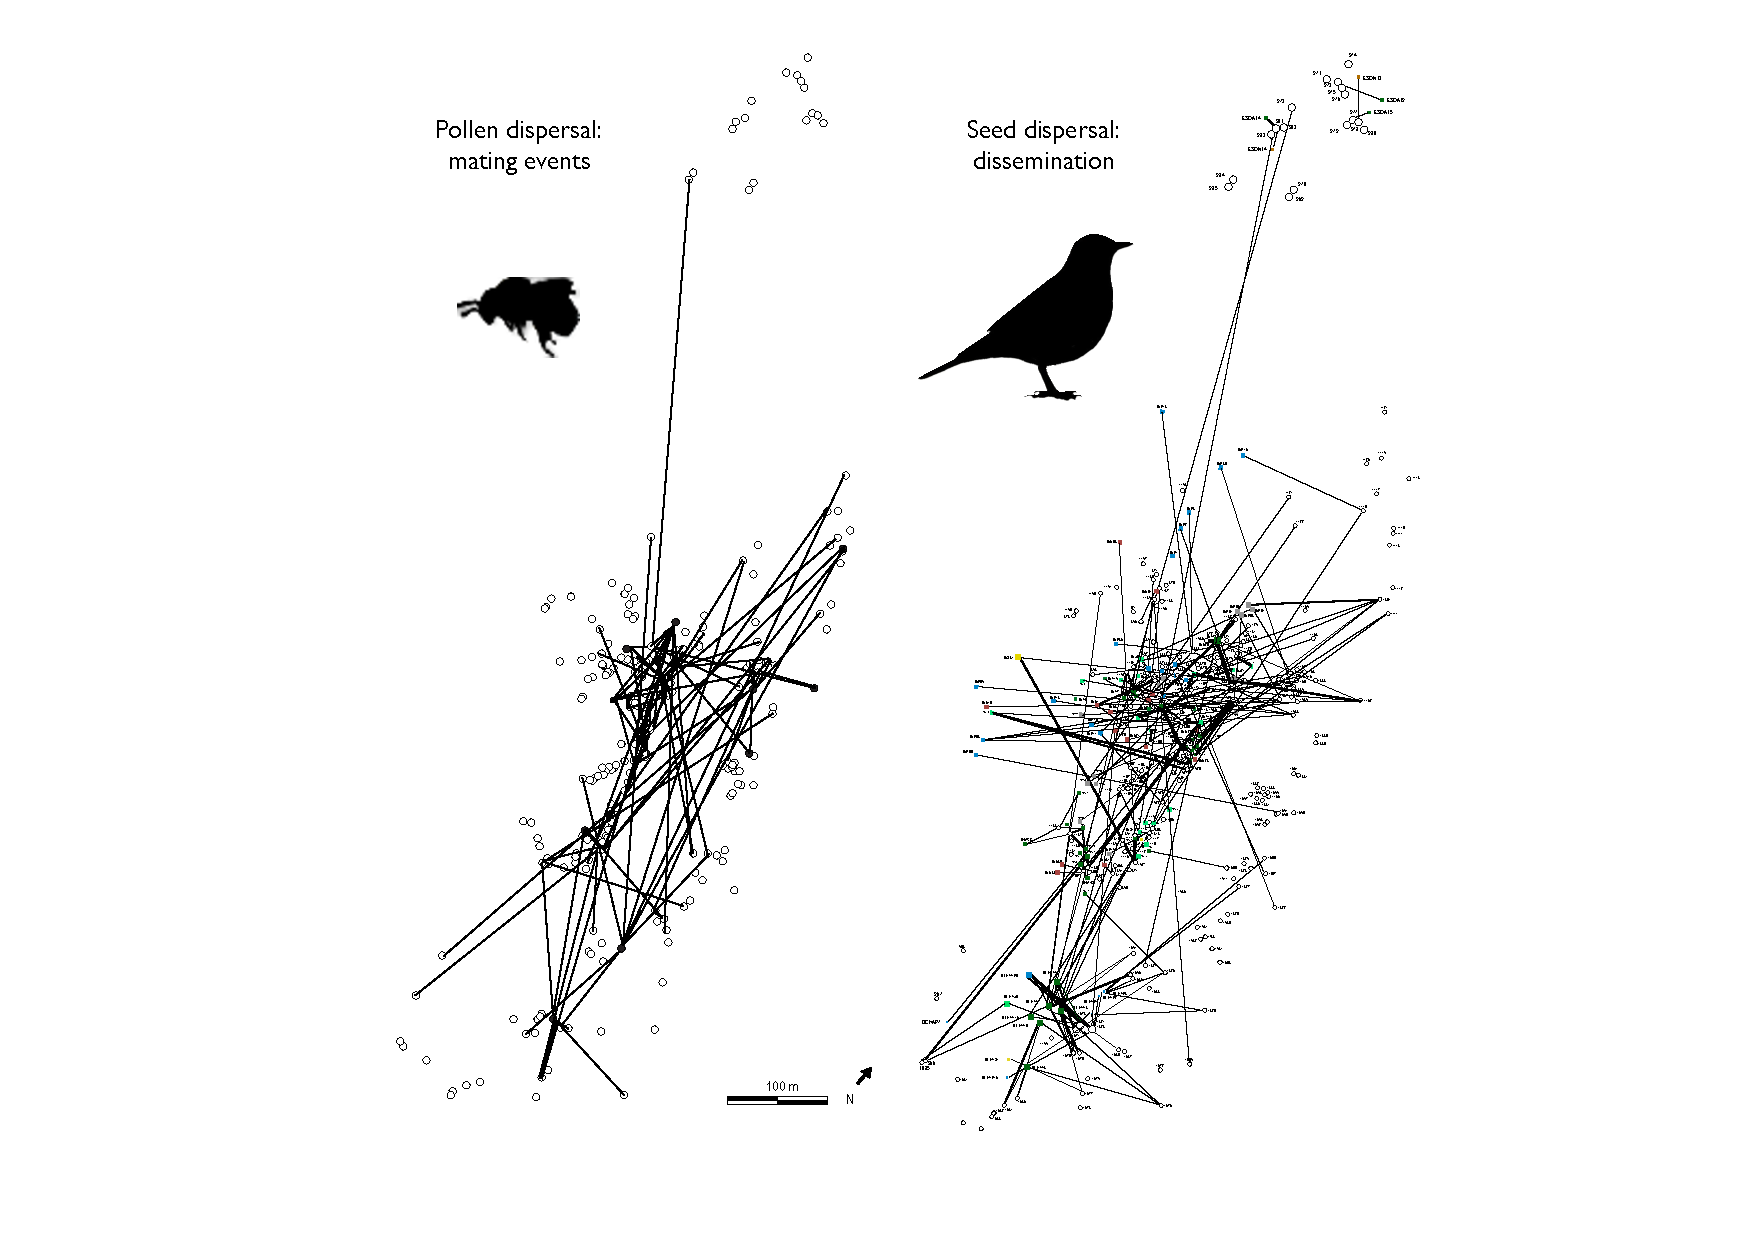
\includegraphics[height=21cm]{FigS1.pdf}}
%
\caption*{Figure S1. Dispersal events for pollen (left) and seeds (right) traced for \textit{Prunus mahaleb} trees (white dots). All the adult, reproductive, trees in the population are mapped. Lines indicate mating events of pollen dispersal among trees (left) or seed dissemination events from source fruiting trees to seed traps (squares; right). Line thickness is proportional to the number of events recorded.}
\end{figure}

\newpage 

%------------------------------------------------------------------ Figure S2
\begin{figure}[htbp]
\centerline{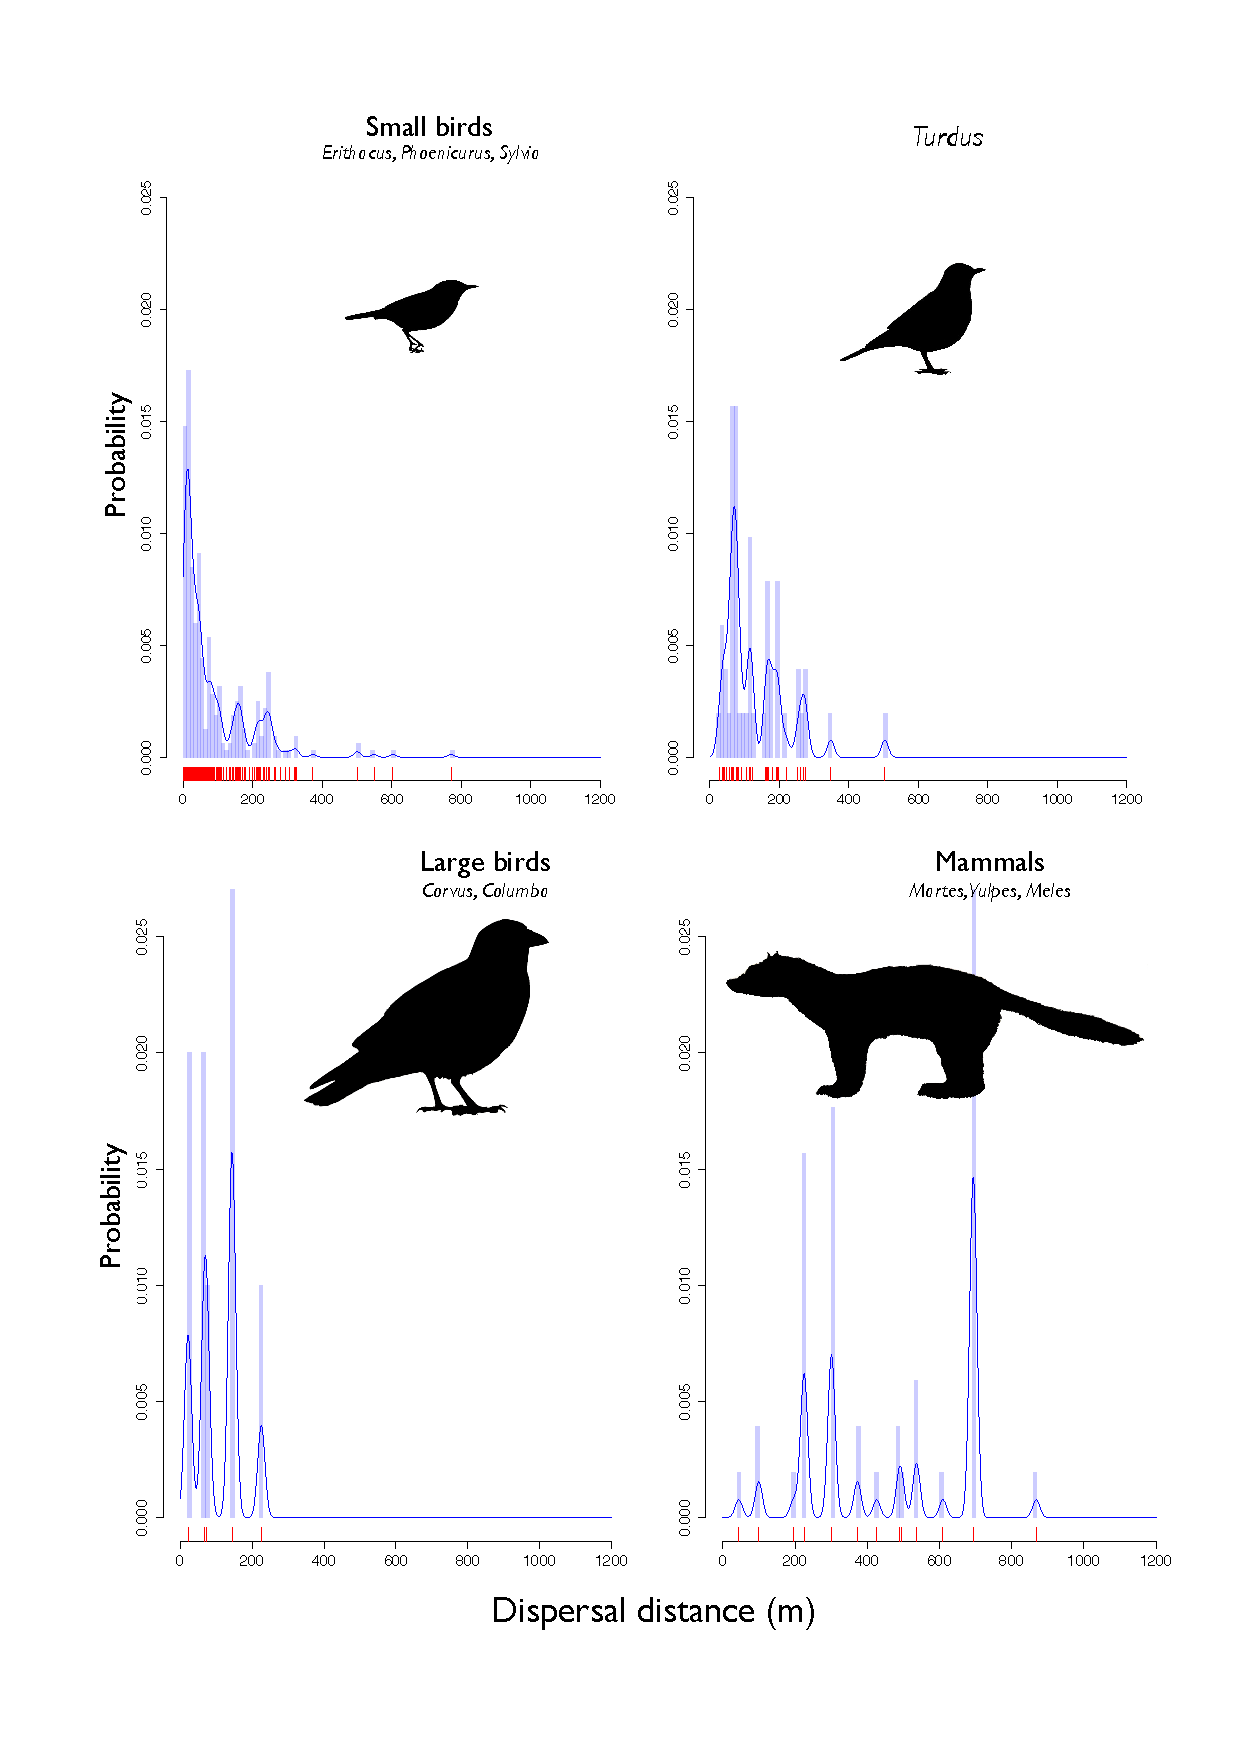
\includegraphics[height=22cm]{FigS2.pdf}}
%
\caption*{Figure S2. Differential contributions of functional groups of frugivores to the short- ($SDD_{loc}$) and long-distance ($LDD_{loc}$) local seed dispersal events for \textit{Prunus mahaleb}.}
\end{figure}

\newpage 

%\section*{References}
%%%%%%%%%%%%%%%%%%%%%%%%%%%%%%%%%%%%%%%%%%%%%%%%%%%%%%%%%%%%%%%%%%%%%%%%%%%%% References
%%% Unnumbered Literature Cited
\bibliographystyle{bes}        %Compile with bes.bst style file
\bibliography{MS_BES}

%%%%%%%%%%%%%%%%%%%%%%%%%%%%%%%%%%%%%%%%%%%%%%%%%%%%%%%%%%%%%%%%%%%%%%%%%%%%%
	
\end{document}
